\newpage
\section{Durchführung}
    \subsection{Versuchsaufbau}
        Für die durchzuführenden Messungen werden drei verschiedene Messaufbauten benötigt, um das Wasserstoffatom, das Wasserstoffmolekül und den 1-dimensionalen Festkörper zu simulieren. 
        \FloatBarrier
        \subsubsection*{Wasserstoffatom}
            Zur Simulation des Wasserstoffatoms wird ein Hohlraumresonator genutzt, der aus zwei aufeinandergesetzten Halbkugeln besteht. In der Wand des Hohlraumresonators befinden sich, wie in 
            Abbildung~\ref{fig:atom_Aufbau} zu sehen, entgegengesetzt ein Mikrofon und ein Lautsprecher. Die Schallwellen des Mikrofons bilden stehende Wellen innerhalb des Hohlraumresonators aus. Die 
            zugehörigen Druckamplituden werden vom Mikrofon vermessen. Zur Änderung der Symmetrieachse kann ein Zwischenring zwischen die beiden Halbkugeln gesetzt werden. Die beiden Halbkugeln können 
            zueinander verdreht werden, sodass der Winkel zwischen dem Mikrofon und dem Lautsprecher zwischen 0° und 180° angepasst werden kann. Für einen Winkel von 180° stehen sich Mikrofon und Lautsprecher
            gegenüber. Es ist darauf zu achten, dass dieser Winkel nicht unbedingt dem tatsächlichen Polarwinkel $\theta$ entspricht. Wenn keine Zwischenringe in das Wasserstoffatom eingesetzt werden muss 
            $\theta$ zunächst berechnet werden:
            \begin{equation*}
                \theta = \arccos\left[\frac{1}{2}\cos\left(\alpha\right) - \frac{1}{2}\right]
            \end{equation*}
            Wenn jedoch Zwischenringe eingesetzt sind steht die Symmetrieachse aufrecht im Hohlraumresonator und der gemessene Winkel entspricht $\theta$.
            \begin{figure}[h]
              \centering
              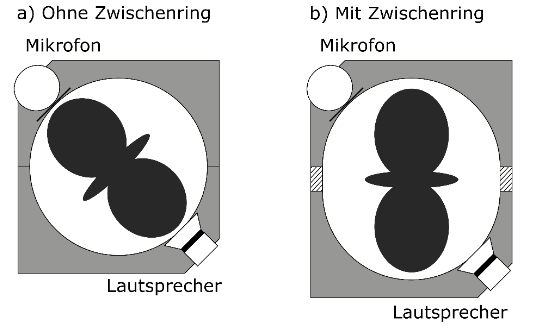
\includegraphics[width = 0.6\textwidth]{pictures/aufbau.png}
              \caption{In der Abbildung ist der Aufbau zur Simulation des Wasserstoffatoms dargestellt. Ein Lautsprecher sendet Schallwellen aus, die von einem Mikrofon auf der entgegengesetzten Seite detektiert werden. Durch das Einsetzen eines Zwischenrings kann die Symmetrieachse verschoben werden. Entnommen aus~\cite{tu_dortmund_versuchsanleitung_2021-4}}
              \label{fig:atom_Aufbau}
            \end{figure}

            \FloatBarrier
        \newpage
        \subsubsection*{Wasserstoffmolekül}
            Um das Wasserstoffmolekül zu simulieren werden nun zwei Kugelresonatoren aufeinandergesetzt. Sie sind durch eine Öffnung in den Kugeloberflächen verbunden. Die Größe dieser Öffnung kann durch 
            Blenden verschiedenen Durchmessers variiert werden. Das Mikrofon und der Lautsprecher befinden sich jeweils in einem der beiden Kugelresonatoren.

        \subsubsection*{1-dimensionaler Festkörper}
            Um das Verhalten eines 1-dimensionalen-Festkörpers zu analysieren, werden Zylinderresonatoren zu Ketten zusammengesetzt. Dabei können verschiedene Zylinderlängen und Blenden genutzt werden, die 
            zwischen den Zylindern platziert werden. Der Lautsprecher wird so angesteuert, dass er über einen Zeitraum mit ansteigender Frequenz einen Ton aussendet. Die entstehenden stehenden Wellen werden 
            vom Mikrofon aufgenommen und entweder wie in Abbildung~\ref{fig:fk_Aufbau} zu sehen über die Steuerelektronik auf das Oszilloskop übertragen oder direkt an einen Computer zur Auswertung mit 
            einem automatischen Programm übertragen. 
            \FloatBarrier

            \begin{figure}[h]
              \centering
              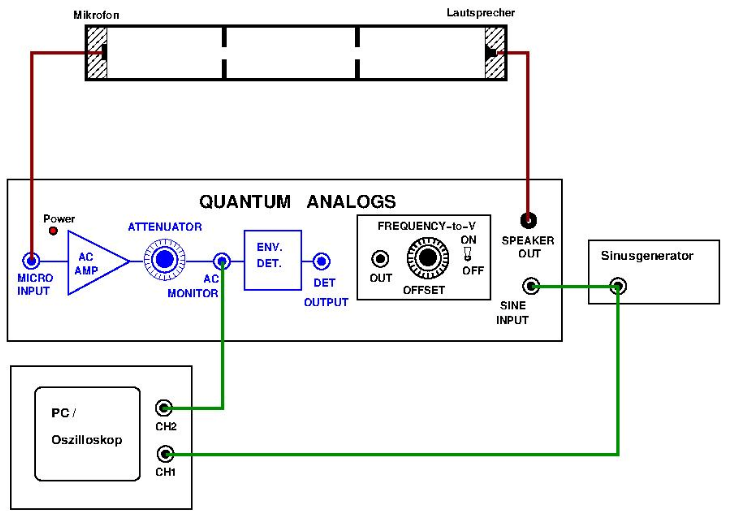
\includegraphics[width = 0.6\textwidth]{pictures/fk_aufbau.png}
              \caption{In der Abbildung ist der Aufbau zur Erzeugung der stehenden Wellen über einen Sinusgenerator und ein Lautsprecher sowie deren Deteḱtion über ein Mikrofon, das das Signal auf ein Oszilloskop oder zum Computer leitet. Entnommen aus~\cite{tu_dortmund_versuchsanleitung_2021-4}}
              \label{fig:fk_Aufbau}
            \end{figure}

            \FloatBarrier

            \noindent


    \subsection{Vorbereitungsmessungen}
        Zur Vorbereitung der späteren Messungen soll zunächst eine Zylinderresonatorkette untersucht werden, die aus Zylinder der Länge \SI{50}{\milli\metre} besteht und im Laufe der Messung von einem auf 12
        Zylinder erweitert werden soll. Für jede Anzahl an Zylindern wird ein Frequenzspektrum der Druckamplitude im Bereich von 0,1 bis \SI{12}{\kilo\hertz} jeweils mit dem Oszilloskop und der 
        Computersoftware aufgenommen. Anschließend werden auch die Frequenzspektren eines einzelnen Zylinders der Länge \SI{50}{\milli\metre} und \SI{75}{\milli\metre} vermessen.

    \subsection{Vermessung des Wasserstoffatoms}
        Zunächst wird ein hochaufgelöstes Frequenzspektrum von 0,1 bis \SI{12}{\kilo\hertz} in \SI{5}{\hertz}-Schritten mit dem Computer aufgenommen. Dabei stehen Mikrofon und Lautsprecher in einem Winkel von 
        180° zueinander und es ist kein Zwischenring eingesetzt.\newline
        Anschließend werden die Resonanzfrequenzen bei gleichem Aufbau mit Hilfe des Oszilloskops bestimmt. Dazu wird die Frequenz des Lautsprechers händisch über den Sinusgenerator von 0,1 bis 
        \SI{100}{\kilo\hertz} variiert. Bei jeder auf dem Oszilloskop sichtbaren Resonanz wird die Ordnung der Resonanz, die Amplitude und die Phasenverschiebung neben der Resonanzfrequenz notiert.\newline
        Für die ausgewählten Resonanzen \SI{2.310}{\kilo\hertz}, \SI{3.711}{\kilo\hertz}, \SI{4.999}{\kilo\hertz} und \SI{7.470}{\kilo\hertz} werden nun hochaufgelöste Spektren für einen Winkelbereich von 
        0° bis 180° in 10°-Schritten aufgenommen.\newline
        Anschließend soll die Aufspaltung der Resonanzfrequenz bei \SI{2.3}{\kilo\hertz} untersucht werden. Dazu werden hochaufgelöste Frequenzspektren in \SI{1}{\hertz}-Schritten zwischen 1,8 und 
        \SI{2.8}{\kilo\hertz} für eingesetzte Zwischenringe der Größen \SI{3}{\milli\metre}, \SI{9}{\milli\metre} und \SI{12}{\milli\metre} aufgenommen.\newline
        Für den \SI{9}{\milli\metre} großen Zwischenring wird die Aufspaltung der Resonanzfrequenz bei \SI{2.3}{\kilo\hertz} in Abhängigkeit des Winkels untersucht, indem hochaufgelöste Spektren der 
        Druckamplituden zwischen 0° und 180° in 10°-Schritten aufgenommen werden.

    \subsection{Vermessung des Wasserstoffmoleküls}
        Zur Untersuchung des Wasserstoffmoleküls werden zunächst hochaufgelöste Frequenzspektren im Bereich zwischen 2,2 und \SI{2.5}{\kilo\hertz} in \SI{1}{\hertz}-Schritten für eingesetzte Blenden der 
        Durchmesser \SI{10}{\milli\metre}, \SI{16}{\milli\metre} und \SI{20}{\milli\metre} aufgenommen.\newline
        Für die \SI{16}{\milli\metre}-Blende wird obriges hochaufgelöstes Frequenzspektrum in Abhängigkeit des Winkels zwischen 0° und 180° in 10°-Schitten aufgenommen. Zusätzlich wird für die dabei 
        auftretenden Resonanzfrequenzen die Phasenverschiebung zwischen der Druckamplitude in der oberen Kugel und der in der unteren Kugel über das Oszilloskop bestimmt.
        
    \subsection{1-dimensionaler Festkörper}
        Zu Beginn wird ein Frequenzspektrum einer Resonatorkette von 0,1 bis \SI{12}{\kilo\hertz} in \SI{5}{\hertz}-Schritten aufgenommen. Das erste Frequenzspektrum wird für eine Kette aus zwei 
        \SI{50}{\milli\metre}-Zylindern, die durch eine \SI{16}{\milli\metre}-Blende getrennt sind, aufgenommen. Daraufhin wird die Kette jeweils um einen Zylinder und eine Blende erweitert, bis die Kette aus 
        zehen Zylindern besteht. Bei jedem nue hinzugefügten Zylinder wird dabei ein Spektrum aufgenommen.\newline
        Daraufhin wird die Messung mit den Blendendurchmessern \SI{10}{\milli\metre} und \SI{13}{\milli\metre} für Ketten aus zwei, vier und 10 Zylindern wiederholt.\newline
        Zur Untersuchung von Fehlstellen wird eine Kette aus 10 \SI{50}{\milli\metre} langen Zylindern mit \SI{16}{\milli\metre}-Blenden aufgebaut. Es werden drei dem ersten entsprechende Frequenzspektren 
        aufgenommen, in denen jeweils einer der \SI{50}{\milli\metre}-Zylinder entweder durch einen \SI{37.5}{\milli\metre}-, \SI{62.5}{\milli\metre}- oder \SI{75}{\milli\metre}-Zylinder ersetzt wurde.\newline
        Anschließend wird eine durch \SI{16}{\milli\metre}-Blenden getrennte Resonatorkette aus 10 Zylindern, die abwechselnd \SI{50}{\milli\metre} und \SI{75}{\milli\metre} lang sind, aufgebaut und wieder 
        das entsprechende Frequenzspektrum aufgenommen.\newline
        Zuletzt wird eine Resonatorkette aus acht \SI{50}{\milli\metre} langen Zylindern aufgebaut, die abwechselnd durch \SI{13}{\milli\metre}- und \SI{16}{\milli\metre}-Blenden getrennt werden. Auch hier 
        wird das Frequenzspektrum im Bereich von 0,1 bis \SI{12}{\kilo\hertz} in \SI{5}{\hertz}-Schritten aufgenommen.


        
        

        
